\section{Multi-User, Multi-World, and Per-Tenant Isolation}
\label{sec:multi-user-worlds}

GAWorld v2 makes a \emph{World} a first-class object.  A world is a city
bundle plus a per-world configuration overlay plus a per-world output root
plus a per-world set of memberships.  The active world is resolved from a
cookie, validated against the caller's role, and propagated through a
context variable.  This section describes the data model, the
request-resolution path, the run-management machinery, the visibility
rules, the static-file guard, and the per-tenant quotas.  When the account
store is absent, the single \texttt{default} world is the only world, and
the system behaves as it did before multi-tenancy was added.

\begin{figure}[t]
  \centering
  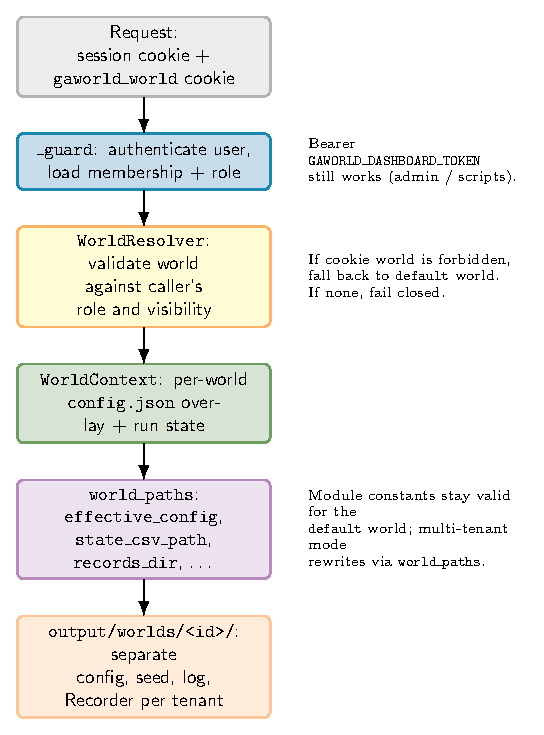
\includegraphics[width=\linewidth]{multi_tenant.pdf}
  \caption{Request resolution in a multi-tenant deployment.  A request enters
  the dashboard server with a session cookie and a \texttt{gaworld\_world}
  cookie; \texttt{\_guard} authenticates the caller, the \texttt{WorldResolver}
  validates the cookie against the caller's role and visibility, and the
  resulting \texttt{WorldContext} drives per-tenant path resolution.}
  \label{fig:multi-tenant}
\end{figure}

\begin{figure}[t]
  \centering
  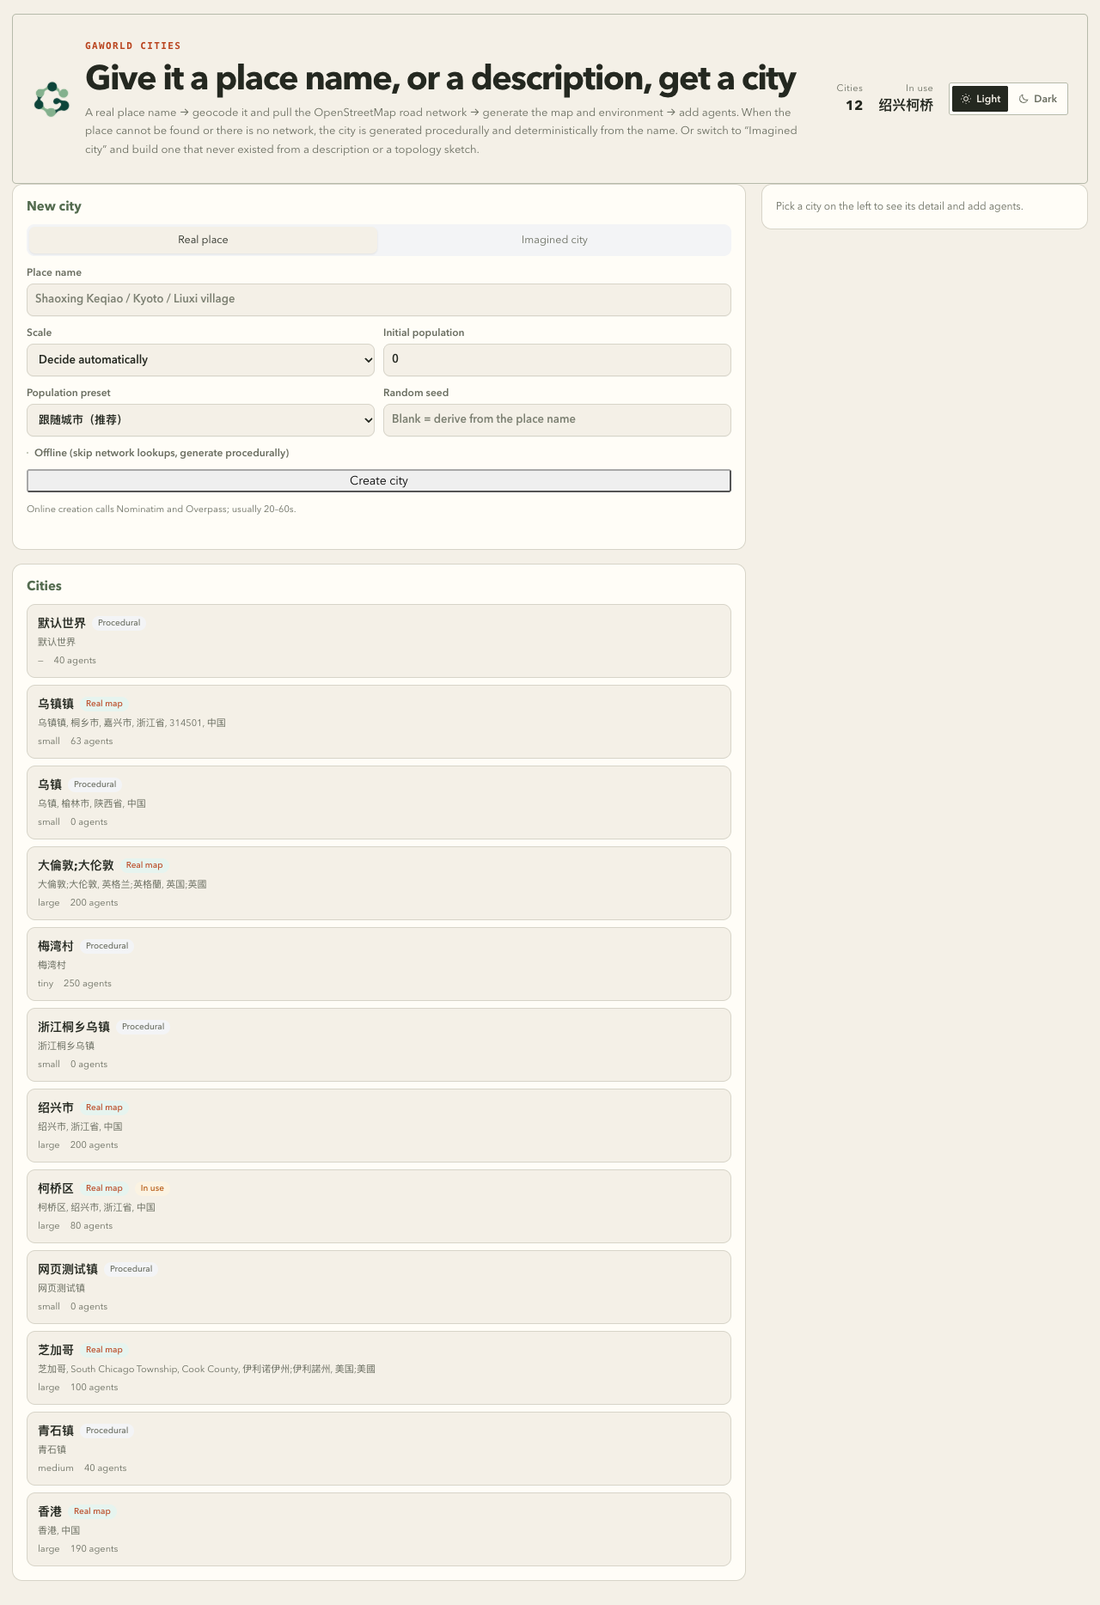
\includegraphics[width=\linewidth]{en_07_citymap.png}
  \caption{The Cities panel.  A v2 deployment lists every city bundle it has
  access to; the panel creates a new city from a real place name (geocoded
  via Nominatim with OpenStreetMap data) or from an imagined description
  (procedurally generated).  Each entry shows the source (\emph{Real map} or
  \emph{Procedural}), the scale (\emph{tiny / small / medium / large}), and
  the agent count.  Selecting a city loads its bundle into the running
  world; the \emph{In use} tag indicates the bundle currently driving the
  active simulation.  This panel is the entry point for per-tenant world
  isolation: when accounts are enabled, each user has a personal \emph{In
  use} pointer and a list of worlds they own or can join.}
  \label{fig:cities}
\end{figure}

\subsection{Data model}

A v2 deployment, when accounts are enabled, stores the following objects in
an SQLite database (\texttt{output/accounts/accounts.sqlite}, no new
dependency):

\begin{itemize}[leftmargin=*]
  \item \textbf{User} with one of two roles: \emph{admin} (teacher) or
  \emph{member} (student), and an optional capability bit
  \texttt{can\_create\_city};
  \item \textbf{Session} storing only a SHA-256 hash of a 32-byte random
  token, with \texttt{HttpOnly; SameSite=Strict} cookies;
  \item \textbf{Invite} generated in batches, optionally labelled, with an
  expiry and a quota template;
  \item \textbf{World} referencing a city bundle, a per-world configuration
  file, and a visibility level;
  \item \textbf{Membership} binding a user to a world as
  \emph{owner}/\emph{player}/\emph{observer};
  \item \textbf{Usage} and \textbf{audit} records for per-tenant quotas and
  forensic replay.
\end{itemize}

A world is a folder under \texttt{output/worlds/\textit{world\_id}/} that
holds the city's \texttt{agents.csv} and \texttt{profiles.md} as
copy-on-write \texttt{seed/} files, the run log, the run-time
configuration overlay, the run state, the intervention queue, and the
Recorder.  When the world is deleted, the folder is removed; when the user
account is deleted, every owned world is deleted with it.  A world is also
the natural unit of distributed execution (see
\Cref{sec:distributed-playable}).

\subsection{Request resolution}

A request enters the dashboard server with a session cookie, a
\texttt{gaworld\_world} cookie indicating the caller's chosen world, and
(optionally) a Bearer token.  The \texttt{\_guard} middleware authenticates
the caller and loads the membership.  The world resolver then:

\begin{enumerate}[leftmargin=*,label=\arabic*.]
  \item reads the caller's \texttt{gaworld\_world} cookie;
  \item verifies that the world exists and that the caller has at least
  \emph{observer} visibility;
  \item if not, falls back to the shared \texttt{default} world (a
  per-tenant deployment may have no such world, in which case the request
  fails closed);
  \item loads the world's \texttt{config.json} and merges it with the global
  \texttt{dashboard\_config.json} under a documented precedence order;
  \item sets a \texttt{ContextVar} that downstream code consults in lieu of
  reading global configuration; and
  \item selects a path-resolving function for the world's output root.
\end{enumerate}

This pattern preserves all module-level path constants in the v1 code:
\texttt{output/} is still the default world's root, and the same code that
reads a relative path in a single-tenant deployment reads a world-rooted
path in a multi-tenant deployment.  Unit tests that monkey-patch module
constants continue to work; the dashboard does not require a new fork
because of multi-tenancy.  A pitfall identified during the migration is
that \texttt{python -m gaworld.apps.dashboard\_server} previously loaded
the module a second time as \texttt{\_\_main\_\_}, producing two parallel
world resolvers.  The fix was to delegate the \texttt{-m} entry point to
the canonical module and to add a regression test
(\texttt{ModuleEntryPointTest}).

\subsection{Path resolution and output isolation}

Without multi-tenancy, the simulation wrote to a fixed set of paths under
\texttt{output/}.  v2 adds a path-resolution layer (\texttt{world\_paths})
that takes a base root and returns the per-world versions of each path.
The base layer is unchanged for the default world, so single-tenant
deployments see no behavior change.  For a multi-tenant deployment, the
path layer reads \texttt{effective\_config} and \texttt{world\_root} from
the context variable and rewrites the \texttt{RUN\_PATHS} entries
(\texttt{memory\_dir}, \texttt{state\_output\_dir}, and
\texttt{kernel.interventions\_path} for the simulation, plus
\texttt{records.output\_dir} and \texttt{records.interventions\_path} for
the dashboard) to the world's root.

A run is launched in the world's process group with
\texttt{GAWORLD\_CONFIG\_OVERRIDES} carrying the world-specific paths.  The
simulation code does not need to know which world it is in; it reads the
override environment variable and writes to the resolved paths.
A configuration change in a world's \texttt{config.json} therefore takes
effect at the next run boundary without restarting the dashboard.

\subsection{Visibility and roles}

A world's visibility is one of \emph{private}, \emph{class}, or
\emph{open}.  A \emph{private} world is visible only to its owner (and any
admin).  A \emph{class} world is read-only for all members; teachers use it
to publish a demonstration world.  An \emph{open} world allows any member
to join; joining creates a \emph{player} membership that lets them claim
residents and act in the simulation.  A \emph{player} can also be downgraded
to an \emph{observer}; an \emph{observer} can read state, profiles, and
memory but cannot mutate anything.

Roles are enforced at the API layer, not at the run layer: the run itself
is unaware of who is watching, but a write to the world is checked against
the caller's role before being applied.  This is the same trust model as
the v1 system but with a finer-grained permission set.

\subsection{Run management and quotas}

A world can have at most one running simulation at a time; the dashboard
also enforces two global limits configurable by the admin:

\begin{itemize}[leftmargin=*]
  \item \texttt{max\_concurrent\_runs} (default 4): the maximum number of
  simulations across all worlds in the deployment;
  \item \texttt{max\_runs\_per\_user} (default 1): the maximum number of
  concurrent simulations per user (admins are exempt).
\end{itemize}

A run request that exceeds a limit is enqueued in a FIFO queue whose head
is the run with the earliest request time; the dashboard reports
``queued (position $k$)'' in the panel.  A user can withdraw a queued
request without affecting other users.  Quotas and queue state persist
across dashboard restarts.

\subsection{Static-file guard}

v2 introduces a static-file guard that requires an authenticated session
cookie to read any path under \texttt{output/} or \texttt{data/}.  The v1
implementation had only a single-token guard and rejected paths whose
basename began with a dot; this was insufficient because a logged-in user
could read other worlds' output.  The v2 guard checks the world
identifier, the caller's role, and the path's owner world before
returning the file.  Static assets outside \texttt{output/} and
\texttt{data/} (CSS, JS, fonts, HTML) are unaffected.

\subsection{Per-tenant ledger and audit}

Every mutation that crosses the API is recorded in the \texttt{audit}
table, with the caller's user id, the world's id, the operation type, the
target entity, and a timestamp.  The audit table is small (one row per
write) and is intended for forensic replay rather than as a primary
trace.  A per-tenant \texttt{usage} table records the number of LLM calls
the tenant has made, broken down by model, by task, and by day.  The
quota system reads from \texttt{usage} and refuses to start a run that
would push the tenant over the daily quota; a configurable dry-run mode
warns without refusing.

\subsection{Backwards compatibility and migration}

The migration to v2 is, by design, backwards compatible.  The
\texttt{AccountStore} is optional: an installation that does not run
\texttt{python -m gaworld.accounts init} continues to behave exactly as
v1 did, with \texttt{GAWORLD\_DASHBOARD\_TOKEN} as the only credential.
A first admin can be created with the same command; from that point on,
\texttt{\_guard} requires a session cookie or a Bearer token, and
\texttt{GAWORLD\_DASHBOARD\_TOKEN} is reserved for scripts and
back-compat.  A migration script exists for installations that want to
adopt multi-tenancy without re-creating their world, but most production
deployments start fresh.  This is the only way to preserve the byte-for-byte
single-tenant behavior that v1 promises; v2's promise is that single-tenant
behavior is preserved exactly when the account store is absent.
